\begin{figure}[t!]
\centering
\vspace*{-1ex}
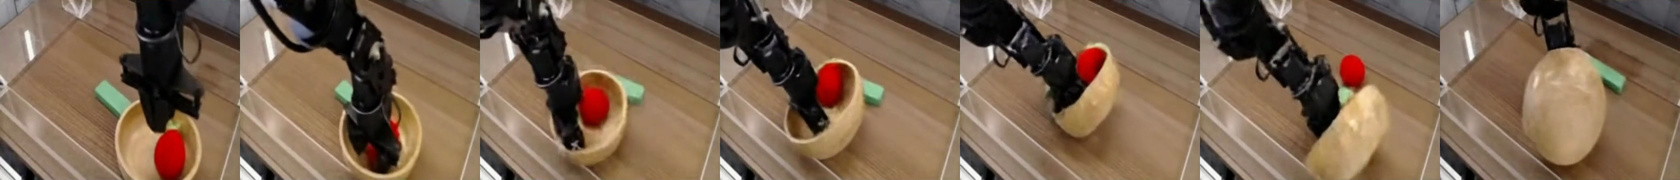
\includegraphics[width=\linewidth]{figures/robotics/soar1} \\[1ex]
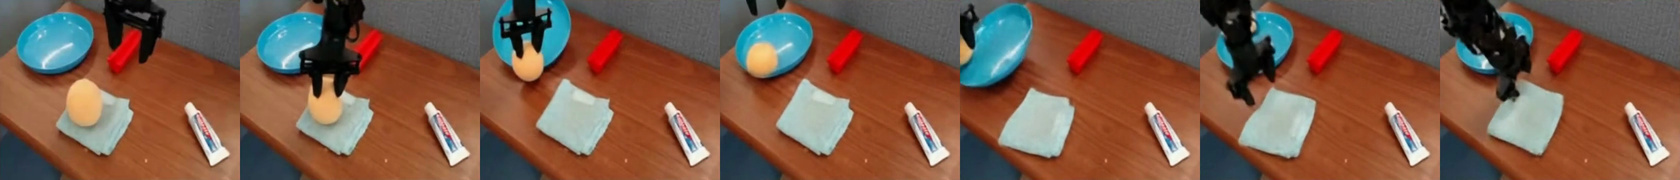
\includegraphics[width=\linewidth]{figures/robotics/soar2} \\[1ex]
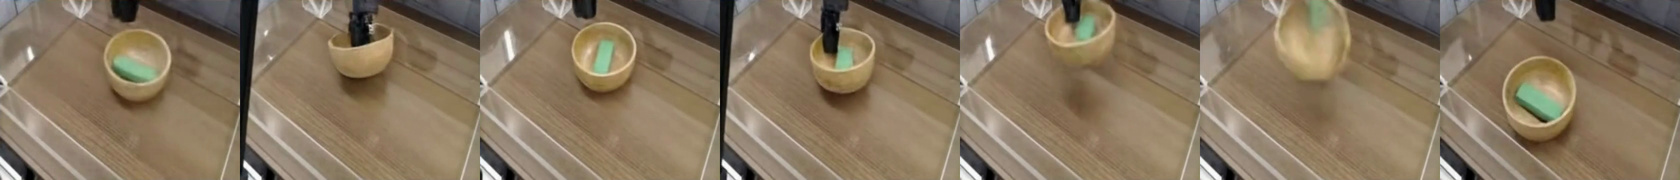
\includegraphics[width=\linewidth]{figures/robotics/soar3}
\caption{
Robotics generations for counterfactual actions.
\method learns an accurate real-time simulator of the environment, allowing human operators to control the imagined robot to pick up objects, flip over a bowl, press a ball onto a plate, move a towel, and throw a bowl.
}
\label{fig:robotics}
\end{figure}
